% ============================================================
%  EWAT — Early Warning and Anomaly Typing
%  Conference-style academic paper (English)
%  Author: Wassim Badraoui — Devoteam internship, 2026
% ============================================================

\documentclass[10pt, twocolumn, a4paper]{article}

% --- Encoding & language ---
\usepackage[utf8]{inputenc}
\usepackage[T1]{fontenc}
\usepackage[english]{babel}

% --- Layout ---
\usepackage[top=2.2cm, bottom=2.2cm, left=1.8cm, right=1.8cm, columnsep=0.7cm]{geometry}

% --- Math ---
\usepackage{amsmath, amssymb, amsthm}
\usepackage{mathtools}

% --- Tables & figures ---
\usepackage{booktabs}
\usepackage{tabularx}
\usepackage{multirow}
\usepackage{graphicx}
\usepackage{float}
\usepackage{caption}
\usepackage{subcaption}
\captionsetup{font=small,labelfont=bf}

% --- Code & algorithms ---
\usepackage{algorithm}
\usepackage{algpseudocode}

% --- Typography ---
\usepackage{microtype}
\usepackage{lmodern}

% --- Links ---
\usepackage[
  colorlinks=true,
  linkcolor=black,
  citecolor=blue,
  urlcolor=blue,
  pdftitle={EWAT — Early Warning and Anomaly Typing},
  pdfauthor={Wassim Badraoui}
]{hyperref}

% --- Symbols ---
\usepackage{pifont}
\newcommand{\cmark}{\textcolor{black}{\ding{51}}}
\newcommand{\xmark}{\textcolor{black}{\ding{55}}}

% --- Bibliography ---
\usepackage[backend=biber, style=numeric, sorting=none]{biblatex}
\addbibresource{bibliography.bib}

% --- Shorthands ---
\newcommand{\St}{\mathbf{S}(t)}
\newcommand{\Gt}{\mathbf{G}(t)}
\newcommand{\R}{\mathbb{R}}
\newcommand{\thetadn}{\theta_{\text{drift}\cap\text{anomaly}}}
\graphicspath{{figures/}}

% ============================================================
\begin{document}

\twocolumn[
\begin{@twocolumnfalse}
\centering
{\LARGE\bfseries EWAT: Early Warning and Anomaly Typing\\[2pt]
in Kubernetes Microservice Architectures\par}
\vspace{0.8em}
{\large Wassim Badraoui\par}
\vspace{0.2em}
{\normalsize Devoteam --- 2026 \quad\textbar\quad \texttt{wassim.badraoui@devoteam.com}\par}
\vspace{1.0em}
\begin{abstract}
\noindent
Kubernetes microservice deployments produce a continuous stream of \emph{benign} change ---
rolling deployments, autoscaling, reconfiguration --- that classical anomaly detectors
confuse with genuine faults, yielding massive false-positive rates in production. We present
EWAT (\emph{Early Warning and Anomaly Typing}), a pipeline that explicitly separates benign
drift from real anomalies before learning an empirical ontology of fault types. EWAT is
positioned as \emph{early warning} (\emph{what} fault, \emph{how long before}) and is
deliberately distinct from root-cause analysis (\emph{where}/\emph{why}, post-mortem).
The four-stage pipeline combines (i) drift detection by Maximum Mean Discrepancy with Random
Fourier Features and a \emph{look-through} mechanism, (ii) a spatio-temporal graph convolutional
encoder, (iii) contrastive siamese typing with agglomerative clustering, and (iv) per-type
precursor classifiers, capped by a formal OWL/RDF ontology built with Transfer Entropy (KSG
estimator). We evaluate on data collected from a real nine-node RKE2 cluster
(\texttt{observit-cluster1}) under controlled Chaos~Mesh fault injection.
We report results with deliberate statistical honesty. Our \textbf{defensible headline is a
macro-AUROC of $0.920$ ($95\%$ bootstrap CI $[0.878, 0.956]$)} for active-scenario typing
against the \emph{independent} Chaos~Mesh ground truth on the \texttt{ewat\_v4\_strat} dataset
--- a deterministic logistic-regression baseline that does \emph{not} require the learned
encoder. The latent space is geometrically structurable (H1: silhouette $=0.782\pm0.065$ over
ten seeds on \texttt{ewat\_v3}). We show that the much higher self-referential precursor AUROC
($0.987\pm0.011$) is \emph{circular} and, via a battery of stress tests, that genuine temporal
precursion exists but only surfaces against the independent target ($\Delta_{\text{far}-\text{near}}=-0.116$).
Negative results are reported as contributions: the look-through hypothesis is robustly
falsified ($p=0.27$ on \texttt{ewat\_v3}, $p=0.37$ on \texttt{ewat\_v4\_strat}), open-set
generalisation to unseen fault types is only partial (OpenMax unknown-AUROC $=0.55$), and the
number of empirical types is intrinsically unstable. End-to-end inference latency is $13$~ms at
the $95$th percentile, $375\times$ under a $5$~s budget.

\smallskip
\noindent\textbf{Keywords:} anomaly detection, early warning, microservices, Kubernetes, STGCN,
Transfer Entropy, concept drift, contrastive typing, open-set recognition.
\end{abstract}

\vspace{1.2em}
\end{@twocolumnfalse}
]

\section{Introduction}
\label{sec:intro}

Microservice architectures deployed on Kubernetes are in permanent flux. Rolling deployments,
horizontal autoscaling, configuration changes and traffic ramps all shift the statistical
distribution of observability signals without any underlying fault. Anomaly detectors that react
to distributional change therefore fire on these \emph{benign drifts} exactly as they fire on
real incidents. We confirm this directly: a per-feature $z$-score detector raises a false alarm
on $100\%$ of benign-drift episodes at every threshold $\sigma\in[2.0,3.5]$ we tested
(Section~\ref{sec:results}). The conflation of drift and anomaly is the operational problem EWAT
attacks.

\paragraph{Early warning, not RCA.}
EWAT is an \emph{early-warning} system: it predicts \emph{what} type of fault is developing and
\emph{how long before} it manifests. It is not root-cause analysis (RCA). RCA is post-mortem and
answers \emph{where} and \emph{why} a failure occurred; EWAT acts \emph{before} the failure and
answers \emph{what} and \emph{when}. Table~\ref{tab:ewat-vs-rca} makes the distinction explicit.
This boundary is a design commitment, not a slogan: the typing and ontology stages approach the
``what'' but never attribute a root cause, and our evaluation metrics (lead time, false-alarm
rate on drifts) are warning metrics, not diagnostic ones.

\begin{table}[t]
\centering
\caption{EWAT (early warning) versus root-cause analysis.}
\label{tab:ewat-vs-rca}
\small
\begin{tabularx}{\columnwidth}{@{}lXX@{}}
\toprule
 & \textbf{EWAT (early warning)} & \textbf{RCA} \\
\midrule
Question & \emph{What} / \emph{when} & \emph{Where} / \emph{why} \\
Timing   & before the fault          & after the fault \\
Output   & typed precursor alert     & causal explanation \\
Metric   & lead time, FA on drift    & localisation accuracy \\
\bottomrule
\end{tabularx}
\end{table}

\paragraph{Four operational regimes.}
A central modelling choice is that we recognise \emph{four} regimes, not three:
$\theta\in\{\theta_{\text{normal}},\theta_{\text{drift}},\theta_{\text{anomaly}},\thetadn\}$.
The fourth regime $\thetadn$ models the faulty-deployment case in which a benign drift and a real
anomaly occur simultaneously --- precisely the case where naive detectors are most dangerous.
The look-through mechanism (Stage~0) is designed to keep the signal flowing during drift rather
than zeroing it out, so that an anomaly hidden inside a drift remains observable.

\paragraph{Contributions.}
\begin{enumerate}\setlength{\itemsep}{1pt}
  \item An atomic, reproducible four-stage early-warning pipeline (Section~\ref{sec:method}),
        implemented as independent testable modules ($425{+}$ unit tests) on a real cluster.
  \item A \emph{geometric} contribution validated as H1: the STGCN latent space is structurable
        into separable fault types, silhouette $=0.782\pm0.065$ over ten seeds
        (Section~\ref{sec:results}), driven by the cosine--average clustering choice on the
        L2-normalised embedding sphere.
  \item A \emph{statistically honest} predictive headline: macro-AUROC $=0.920$
        $[0.878,0.956]$ for active-scenario typing against the independent Chaos~Mesh ground
        truth, deterministic and without the learned encoder.
  \item Evidence, via a stress-test battery (Section~\ref{sec:validity}), that the
        self-referential precursor AUROC ($0.987$) is \emph{circular}, while genuine temporal
        precursion exists against the independent target ($\Delta_{\text{far}-\text{near}}=-0.116$).
  \item Reported \emph{negative} results as contributions: look-through falsified twice
        ($p=0.27$, $p=0.37$), partial open-set recognition (OpenMax $0.55$), unstable type count.
  \item A formal OWL/RDF ontology of fault types (29 literature-anchored classes, 143
        individuals, HermiT-consistent) extracted with multivariate Transfer Entropy (KSG), never
        Granger causality.
\end{enumerate}

All numbers in this paper are traceable to the project's experiment logs; we name the dataset and
configuration for every figure, and we surface --- rather than hide --- the residual
inconsistencies we found between intermediate runs (Section~\ref{sec:limitations}).

\section{Related Work}
\label{sec:related}

\paragraph{RCA for microservices.}
The dominant body of work on microservice reliability targets root-cause analysis. Fu et
al.~\cite{fu2025} survey the field and identify a persistent gap between benchmark performance and
production deployability, driven largely by false positives. Soldani and Brogi~\cite{soldani2022}
catalogue microservice anti-patterns and failure modes; we reuse their taxonomy, together with
Gregg's USE methodology~\cite{gregg2013} and cascading-failure modelling~\cite{aniello2014}, to
anchor our OWL class hierarchy in the literature rather than in ad-hoc cluster labels. EWAT
departs from this line of work in objective: we predict and type developing faults rather than
explaining past ones.

\paragraph{Concept drift.}
Distinguishing benign distributional change from genuine anomalies is a concept-drift problem.
Hinder et al.~\cite{hinder2024} formalise drift in unsupervised streams, and Myrtollari et
al.~\cite{myrtollari2025} propose drift-aware anomaly detection specifically for Kubernetes
microservices. EWAT operationalises the drift/anomaly separation as an explicit fourth regime
$\thetadn$ and a look-through filter built on the kernel two-sample test~\cite{gretton2012},
estimated cheaply with Random Fourier Features. Our negative result on look-through
(Section~\ref{sec:validity}) is, to our knowledge, a useful data point on the limits of MMD-based
separation on short episodes.

\paragraph{Representation learning on service graphs.}
We encode the time-evolving service graph with a spatio-temporal graph convolutional network
(STGCN)~\cite{yu2018}, and compare against graph attention~\cite{velivckovic2018} and contrastive
pre-training in the SimCLR style~\cite{chen2020simclr}. Type structure is assessed with the
silhouette criterion, using the conventional acceptability threshold of $0.3$~\cite{kaufman1990},
complemented by the gap statistic~\cite{tibshirani2001} for choosing the number of clusters.

\paragraph{Causality and interpretability.}
For the ontology we estimate directed information flow with Transfer Entropy using the KSG
estimator~\cite{kraskov2004} --- never Granger causality, which assumes linearity inappropriate
for our signals --- and control multiple testing with Benjamini--Hochberg FDR~\cite{benjamini1995}.
Feature attributions are validated with SHAP~\cite{lundberg2017} after we found gradient-based
saliency to be unreliable ($\rho=-0.34$ against permutation importance).

\paragraph{Open-set recognition.}
Because production faults include types never seen in training, we evaluate open-set recognition
with OpenMax~\cite{bendale2016openmax} and discuss Mahalanobis~\cite{lee2018mahalanobis} and
energy-based~\cite{liu2020energy} alternatives as future work. For external validation we adapt
the public RCAEval RE2-OB benchmark~\cite{rcaeval}.

\section{Problem Formalisation}
\label{sec:formal}

\subsection{Service graph}
We model the system as a time-evolving weighted graph $\Gt=(V,E(t),w_E(t))$. Vertices $V$ are
Kubernetes \emph{services} and \emph{deployments} (not pods), with $|V|=N$ held constant over an
episode. Each edge carries a vector weight $w_E(t):E(t)\to\R^3$,
$e_{ij}(t)\mapsto(\text{volume}_{ij},\text{latency}^{\text{med}}_{ij},\text{error-rate}_{ij})$; an
edge is present when its call volume exceeds zero over the sliding window.

\subsection{Telemetry signal}
The per-step signal stacks three modalities,
\begin{equation}
\St=\big[\,\mathbf{M}(t)\;\big|\;\mathbf{T}(t)\;\big|\;\mathbf{L}(t)\,\big]\in\R^{N\times 17},
\end{equation}
with $\mathbf{M}(t)\in\R^{N\times7}$ metrics (CPU, RAM, latency P99, HTTP error rate, network
saturation, disk I/O, queue depth), $\mathbf{T}(t)\in\R^{N\times6}$ trace features (span-duration
P99, abnormal-span rate, trace depth, fan-out, retry rate, latency coefficient of variation), and
$\mathbf{L}(t)\in\R^{N\times4}$ log features (error rate, warning rate, semantic anomaly score as
mean SentenceBERT distance to the normal centroid, lexical entropy). Metrics come from the
existing Prometheus stack; traces and logs from the OpenTelemetry collector. Crucially,
$\St\sim D_{\theta(t)}(\Gt)$ is \emph{not} an additive mixture of regime effects.

\paragraph{Differentiated aggregation.}
Intra-service aggregation is component-specific, never a plain mean: saturation components (CPU,
RAM, net, disk I/O) aggregate by \emph{max}; rate components (error, warning) by
\emph{volume-weighted sum}; latency components (P99, span duration) by the \emph{P99 of the union}
of raw per-pod distributions (never a percentile of percentiles); structural components (trace
depth, fan-out, lexical entropy) by \emph{median}.

\subsection{Operational regimes}
The regime variable is $\theta(t)\in\{\theta_{\text{normal}},\theta_{\text{drift}},
\theta_{\text{anomaly}},\thetadn\}$. Table~\ref{tab:regimes} gives the correspondence to dataset
labels. Benign drift $\theta_{\text{drift}}$ (rolling deploy, autoscaling) is \emph{not} a regime
label; it is detected orthogonally by the drift detector through the boolean
\texttt{drift\_flag}. The combined regime $\thetadn$ is materialised by the
\texttt{faulty\_deploy\_overlap} scenario.

\begin{table}[t]
\centering
\caption{Regime $\theta$ to dataset label correspondence (\texttt{labels.parquet}).}
\label{tab:regimes}
\small
\begin{tabularx}{\columnwidth}{@{}lX@{}}
\toprule
\textbf{Label} & \textbf{Regime} \\
\midrule
\texttt{normal}        & $\theta_{\text{normal}}$ (pre-injection reference) \\
\texttt{injection}     & $\theta_{\text{anomaly}}$ (chaos active) \\
\texttt{drift\_anomaly}& $\thetadn$ (simultaneous faulty deploy) \\
\texttt{recovery}      & post-injection return (excluded from H1/H3) \\
\texttt{drift\_flag}   & $\theta_{\text{drift}}$ (detected, not a label) \\
\bottomrule
\end{tabularx}
\end{table}

\subsection{Hypotheses and falsification}
\label{sec:hypotheses}
EWAT is organised around four falsifiable hypotheses.
\textbf{H1 (structurability).} Fault types form separable groups in the latent space; falsified if
held-out silhouette $<0.3$~\cite{kaufman1990} across seeds and splits.
\textbf{H2a (drift separability).} Look-through reduces the false-positive rate at constant recall;
falsified if no significant reduction ($p>0.05$).
\textbf{H2b (combined-regime identification).} The pipeline identifies $\thetadn$ as distinct from
pure drift and pure anomaly; falsified if no cluster shows simultaneous
\texttt{drift\_flag} and precursor alert above chance.
\textbf{H3 (predictability).} Per-type precursors beat the $0.5$ baseline for some horizon $k$;
falsified if AUROC $<0.5\;\forall k$. We additionally distinguish \emph{circular} H3
(self-referential cluster labels as target) from \emph{honest} H3 (independent Chaos~Mesh
scenarios as target), a distinction that turns out to be decisive (Sections~\ref{sec:results}
and~\ref{sec:validity}).

\section{Method}
\label{sec:method}

EWAT is a cascade of four stages (Figure~\ref{fig:pipeline}); stages~0, 1 and 3 run online within a
latency budget, while typing and ontology construction (stage~2/2b) run offline.

\begin{figure}[t]
\centering
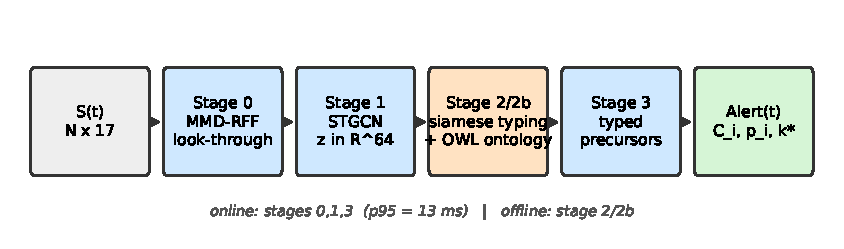
\includegraphics[width=\columnwidth]{pipeline_architecture.pdf}
\caption{The EWAT four-stage pipeline. Stage~0 (drift), stage~1 (encoder) and stage~3
(precursors) are online; stage~2/2b (typing and ontology) are offline.}
\label{fig:pipeline}
\end{figure}

\subsection{Stage 0 --- Drift detection (MMD-RFF, look-through)}
We estimate $\text{MMD}^2(W_{\text{ref}},W_{\text{cur}})$ between a reference and a current window
with Random Fourier Features $\varphi:\R^d\to\R^D$, giving $O(nD)$ cost. The \emph{look-through}
filter never zeroes the signal during drift:
if $\text{MMD}^2<\varepsilon_{\text{drift}}$ the signal passes unchanged; if it exceeds the
threshold and a post-drift confirmation test is positive, the signal passes flagged
\texttt{DRIFT}; if the confirmation is negative, the detector recalibrates
($W_{\text{ref}}\!\leftarrow\!W_{\text{cur}}$). The threshold is calibrated by injecting benign
drifts; we obtain $\varepsilon_{\text{drift}}=0.5226$ (Youden-optimal).

\subsection{Stage 1 --- STGCN encoder}
The encoder maps a windowed signal and graph to an embedding
$z_e=\mathrm{Enc}_\theta(\tilde{\mathbf{S}}_{[t-W,t+\delta]},\Gt)\in\R^{64}$, combining graph
convolution over the weighted adjacency with a causal temporal-convolution stack and a masked
mean-pooling head (padding excluded). It is pre-trained by self-supervised reconstruction without
scenario labels. The graph convolution uses the time-varying adjacency $A(t)$ (the earlier static
$A_{\text{mean}}$ implementation is retained only as an ablation variant).

\subsection{Stage 2 --- Contrastive typing}
A siamese projection head ($d_{\text{proj}}=64$) trained with a contrastive hinge loss
(margin~$2.0$, semi-hard negative mining) maps embeddings onto the L2-normalised unit sphere.
Because the embeddings live on a sphere, we cluster with \emph{average-linkage agglomerative
clustering under cosine distance} --- aligning the metric with the geometry, a change that proves
to be the principal driver of H1 (Section~\ref{sec:results}). Cross-split labels are assigned by
\emph{nearest centroid} from the training centroids, so cluster identities are consistent across
train/val/test. Per-type feature attributions use permutation importance, cross-validated with
KernelSHAP~\cite{lundberg2017}.

\subsection{Stage 2b --- Ontology}
The ontology $O=(C,R)$ carries three relation families: temporal transitions
$C_i\!\to^{\Delta t,\sigma}\!C_j$; \emph{causal} edges from Transfer Entropy with the KSG
estimator~\cite{kraskov2004} (multivariate on synthesised cascades; permutation-bootstrap
significance with Benjamini--Hochberg FDR~\cite{benjamini1995}); and co-occurrence edges by a
$2\times2$ Yates $\chi^2$ with a Fisher-exact fallback and Holm correction. The result is exported
as a formal OWL/RDF artefact (TBox of 29 literature-anchored classes; ABox of 143 individuals) and
checked for consistency with the HermiT reasoner.

\subsection{Stage 3 --- Typed precursors}
For each type $C_i$ a one-vs-rest classifier produces a precursor probability
$\hat{p}_i(t)=f_i(\tilde{\mathbf{S}}_{[t-k,t]},\Gt)\in[0,1]$. The horizon is chosen \emph{on the
validation set}, $k^*_i=\arg\max_k \mathrm{AUROC}(f_i,k)$ over $k\in\{1,\dots,20\}$ steps; test
AUROC is reported only at $k^*_i$. The final alert is
$\mathrm{Alert}(t)=(C_i,\hat{p}_i(t),k^*_i,\text{card}_{C_i})$.

\subsection{Latency budget}
The formal budget is stage~0 $<1$~s, stage~1$+$2 $<2$~s, stage~3 $<1$~s, total $<5$~s. Measured on
CPU over 200 iterations (Table~\ref{tab:latency}), the end-to-end $95$th percentile is $13.28$~ms
--- $375\times$ under budget.

\begin{table}[t]
\centering
\caption{End-to-end inference latency (CPU, 200 iterations, \texttt{ewat\_v3}).}
\label{tab:latency}
\small
\begin{tabularx}{\columnwidth}{@{}Xrrr@{}}
\toprule
\textbf{Stage} & \textbf{median} & \textbf{p95} & \textbf{budget} \\
\midrule
0 — drift               & 0.01~ms & 0.01~ms & 1000~ms \\
1+2 — encoder+siamese   & 0.96~ms & 1.97~ms & 2000~ms \\
3 — precursors          & 1.85~ms & 3.91~ms & 1000~ms \\
\midrule
\textbf{Total}          & \textbf{9.26~ms} & \textbf{13.28~ms} & \textbf{5000~ms} \\
\bottomrule
\end{tabularx}
\end{table}

\section{Experimental Setup}
\label{sec:setup}

\paragraph{Cluster and observability.}
All data were collected on \texttt{observit-cluster1}, a real nine-node RKE2 cluster (Kubernetes
v1.32.7) running the Online Boutique demo. Two observability stacks coexist: Prometheus/Grafana
for mature metrics and an OpenTelemetry collector for traces and logs, correlated through OTel
semantic conventions. The service set is fixed at $N=6$ (\texttt{frontend}, \texttt{cart},
\texttt{recommendation}, \texttt{ad}, \texttt{product-catalog}, \texttt{load-generator}); services
invisible on any modality were excluded to avoid systemic NaNs.

\paragraph{Fault injection.}
Faults are injected with Chaos~Mesh over 15 scenarios: 4 benign drifts
(\texttt{drift\_config\_change}, \texttt{drift\_rolling\_deploy}, \texttt{drift\_scale\_up},
\texttt{drift\_traffic\_ramp}) and 11 anomalies, including \texttt{faulty\_deploy\_overlap} which
realises the combined regime $\thetadn$. Each episode follows the
\emph{record\,$\to$\,build\,$\to$\,assemble} protocol: raw dumps are immutable ground truth,
features are recomputed offline, and datasets are split last.

\paragraph{Datasets.}
Table~\ref{tab:datasets} summarises the four datasets. We highlight one methodological pitfall:
the original temporal split of \texttt{ewat\_v4} left four scenarios entirely absent from the
training set, collapsing the independent-target AUROC to a trivial $0.5$. We therefore assembled
\texttt{ewat\_v4\_strat} (stratified, at least one episode per scenario per split), which is the
dataset behind our defensible headline.

\begin{table}[t]
\centering
\caption{Datasets. ``strat'' = stratified split guaranteeing every scenario in every split.}
\label{tab:datasets}
\small
\begin{tabularx}{\columnwidth}{@{}lXl@{}}
\toprule
\textbf{Dataset} & \textbf{Episodes / split} & \textbf{Notes} \\
\midrule
\texttt{ewat\_v3}       & 299; 209/45/45 (strat) & $\sim$21 steps; disk\_io 16.7\% NaN \\
\texttt{ewat\_v4}       & 375; 262/56/57 (temp.) & 47--51 steps; 4 scen.\ absent train \\
\texttt{ewat\_v4\_strat}& 270/60/45 (strat)      & \textbf{headline dataset} \\
\texttt{ewat\_rcaeval}  & 90; 30 fault types     & adapted RCAEval RE2-OB \\
\bottomrule
\end{tabularx}
\end{table}

\paragraph{Protocol and methodology corrections.}
Unless stated otherwise, H1/H3 on \texttt{ewat\_v3} use the optimised configuration
(average$+$cosine clustering, $d_{\text{proj}}=64$, margin~$2.0$, tuned logistic regression) and
are aggregated over ten seeds. Two methodological corrections apply throughout: (i) H1 silhouette
on val/test is computed with \emph{nearest-centroid} labels from the training centroids, not an
independent per-split clustering (which inflated scores); (ii) the precursor horizon $k^*$ is
selected on validation, never on test. Confidence intervals are $95\%$ bootstrap (BCa for AUROC).
We name the dataset and configuration for every reported number, because they differ
substantially between \texttt{ewat\_v3} and \texttt{ewat\_v4\_strat}.

\section{Results}
\label{sec:results}

We organise results by hypothesis, then report baselines, ablations, architecture comparison,
ontology, and operational alerting. Throughout we separate the \emph{circular} evaluation target
(EWAT's own cluster labels) from the \emph{independent} target (Chaos~Mesh scenarios); only the
latter supports a defensible predictive claim.

\subsection{H1 --- Structurability (PASS)}
On \texttt{ewat\_v3} with the optimised configuration, the held-out silhouette is
$0.782\pm0.065$ over ten seeds (minimum $0.618$, all $\gg 0.3$): H1 passes robustly. The optimised
configuration improves on the initial baseline (Ward$+$Euclidean, $0.519\pm0.092$) by $+51\%$; the
gain is geometric and comes almost entirely from matching the clustering metric (cosine) to the
L2-normalised embedding sphere. On the longer \texttt{ewat\_v4\_strat} episodes the silhouette is
lower and more variable ($0.691\pm0.115$, range $[0.521,0.839]$), and the number of types $K$ is
intrinsically unstable: neither silhouette nor the gap statistic stabilises it (modes $K=14$ and
$K=12$ respectively, agreement on only $4/10$ seeds). Figure~\ref{fig:multiseed} shows the
per-seed distributions.

\begin{figure}[t]
\centering
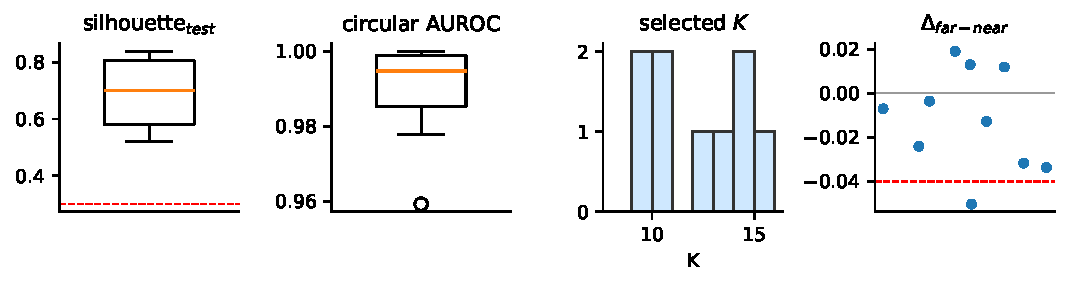
\includegraphics[width=\columnwidth]{multiseed_distribution.pdf}
\caption{Multi-seed distributions (\texttt{ewat\_v4\_strat}, Phase~H, 10 seeds): silhouette,
circular precursor AUROC, selected $K$, and the distant-window gap $\Delta$. The circular AUROC is
stable; silhouette, $K$ and $\Delta$ are not, and seed~42 is an outlier on $\Delta$.}
\label{fig:multiseed}
\end{figure}

\subsection{H2a --- Drift separability by look-through (FAIL)}
Look-through does not reduce the false-positive rate. On \texttt{ewat\_v3}, the look-through
detector reaches a drift true-positive rate of $0.42$ versus $0.67$ for a plain threshold, and an
anomaly false-positive rate of $0.67$ versus $0.73$ --- not a significant reduction
($p=0.27$, paired one-sided $t$). The same test on STGCN embeddings is also negative
($p=0.978$). Critically, the negative result is \emph{robust} to episode length: re-running on the
$2\times$ longer \texttt{ewat\_v4\_strat} episodes still fails ($\text{TPR}=0.50$, $p=0.372$).
The mechanism is falsified, not merely under-powered; we report this as an honest negative result.

\subsection{H2b --- Combined regime $\thetadn$ (PASS but trivial)}
The formal criterion passes (overlap $>30\%$ everywhere), but trivially: the drift detector's
5-step window fires on almost every short episode, so overlap is high regardless. A strict Fisher
test of the overlap cluster (\texttt{faulty\_deploy\_overlap}) against pure drift gives
$\text{OR}=1.48$, $p=0.35$ --- not significant. Moreover, the precursor alert \emph{precedes} the
drift flag in $85$--$100\%$ of cases: the drift detector is a \emph{late} indicator, and the early
warning comes from stage~3, not stage~0. H2b thus reinforces H2a rather than standing on its own.

\subsection{H3 --- Predictability}
\paragraph{Circular target (self-referential).}
Predicting EWAT's own cluster labels from the embedding gives a peak AUROC of $0.987\pm0.011$
($10/10$ seeds PASS). We flag this as \emph{circular}: the target is produced by the same
encoder/clustering being evaluated. Section~\ref{sec:validity} shows directly that this number does
not reflect temporal precursion.

\paragraph{Independent target (honest).}
Against the Chaos~Mesh ground truth, our defensible headline is a deterministic logistic-regression
one-vs-rest classifier on instance-normalised pre-injection features (no learned encoder):
\textbf{macro-AUROC $=0.920$, $95\%$ bootstrap CI $[0.878,0.956]$} on
\texttt{ewat\_v4\_strat}, stable under leave-one-scenario-out ($0.930\pm0.007$, 15 folds).
Table~\ref{tab:baselines} consolidates all baselines by target. Two facts stand out: the encoder
does \emph{not} add aggregate predictive value (training an STGCN end-to-end on the same
independent target yields $0.863$, \emph{below} the linear baseline), and the circular numbers
($0.95$--$0.99$) sit far above the honest ones ($0.84$--$0.94$).

\begin{table}[t]
\centering
\caption{Baselines grouped by evaluation target. Circular = EWAT's own labels; Independent =
Chaos~Mesh scenarios. CIs are $95\%$ bootstrap.}
\label{tab:baselines}
\small
\begin{tabularx}{\columnwidth}{@{}Xl@{}}
\toprule
\textbf{Model (dataset)} & \textbf{macro-AUROC} \\
\midrule
\multicolumn{2}{@{}l}{\emph{Circular target — EWAT cluster labels}}\\
Random                                    & 0.500 \\
Raw features $\to$ EWAT labels (v3)        & 0.966 \\
$k$-means + LR $\to$ EWAT labels (v3)      & 0.975 \\
EWAT precursors, self (v3)                 & 0.951 \\
EWAT precursors, optimised peak (v3, 10s)  & $0.987\pm0.011$ \\
\midrule
\multicolumn{2}{@{}l}{\emph{Independent target — Chaos~Mesh scenarios}}\\
Raw features, $k{=}6$ (v3)                 & 0.835 {\scriptsize[0.773,0.888]} \\
STGCN $z_e$ (v3)                           & 0.835 {\scriptsize[0.772,0.885]} \\
STGCN end-to-end (v4\_strat)               & 0.863 {\scriptsize[0.823,0.905]} \\
Raw, instance-norm best (v4\_strat)        & 0.941 {\scriptsize[0.909,0.970]} \\
\textbf{Raw, inst-norm flatten LR (v4\_strat)} & \textbf{0.920} {\scriptsize[0.878,0.956]} \\
\bottomrule
\end{tabularx}
\end{table}

\paragraph{Per-scenario redistribution.}
On \texttt{ewat\_v3} the aggregate gap between raw features and STGCN embeddings is exactly
$\Delta_{\text{macro}}=0.000$. This is not neutrality by coincidence alone: AUROC on $n=45$ test is
a ratio of concordant pairs over a fixed integer denominator, and the encoder \emph{redistributes}
discriminability across scenarios (e.g.\ $+27$~pp on \texttt{fail\_slow\_cpu}, $-25$~pp on
\texttt{noisy\_neighbor}) with the per-scenario gains and losses summing to zero. The redistribution
is real; its exact cancellation is an artefact of the small test set.

\subsection{Ablations}
\paragraph{Modality (rigorous, full retraining).}
Retraining the encoder and siamese head per condition (seed 42, \texttt{ewat\_v3}),
metrics-only beats the full model on H1 silhouette ($0.497$ vs $0.439$, $\Delta=+0.058$); adding
traces and logs injects geometric noise into the clustering on $n=209$. Logs-only collapses
($0.051$). The hierarchy is $M>T>L$ for clustering geometry.\footnote{An inference-time masking
ablation (no retraining) gives a lower full baseline of $0.333$ but the same qualitative ranking;
we report the rigorous retraining figures here.}
\paragraph{Modality (precursor H3, inference masking).}
For predictability the ordering inverts: the full model is best ($0.954$), and dropping traces and
logs hurts ($M$-only $0.756$, $L$-only $0.488$). Traces and logs are noise for clustering geometry
but \emph{necessary} for prediction. The single most critical feature for H3 is \texttt{disk\_io}
($\Delta=-0.088$ leave-one-out), despite its $16.7\%$ NaN rate --- a direct argument for the
\texttt{ewat\_v4} re-collection. Two feature pairs are redundant
($|\rho|>0.9$): \texttt{latency\_p99}$\leftrightarrow$\texttt{span\_dur\_p99} and
\texttt{error\_rate\_http}$\leftrightarrow$\texttt{abnormal\_span\_rate}.

\subsection{Encoder architecture comparison}
Table~\ref{tab:arch} compares encoders on \texttt{ewat\_v3} (seed 42, corrected methodology). GAT
gives the best clustering geometry and type coverage; SimCLR the best circular AUROC; STGCN the
most stable $K$. We retain STGCN as the reference (simplest, multi-seed evidence available), while
noting that none of these encoders improves the \emph{independent}-target prediction
(Section~\ref{sec:validity}).

\begin{table}[t]
\centering
\caption{Encoder comparison (\texttt{ewat\_v3}, seed 42). AUROC is the circular precursor metric.}
\label{tab:arch}
\small
\begin{tabularx}{\columnwidth}{@{}Xrrrr@{}}
\toprule
\textbf{Encoder} & $K$ & \textbf{sil$_{\text{test}}$} & \textbf{types} & \textbf{AUROC} \\
\midrule
STGCN  & 10 & 0.414 & 8/10  & 0.954 \\
SimCLR & 15 & 0.429 & 11/15 & \textbf{0.964} \\
GAT    & 15 & \textbf{0.497} & \textbf{13/15} & 0.929 \\
\bottomrule
\end{tabularx}
\end{table}

\subsection{Ontology}
The OWL/RDF ontology comprises 29 literature-anchored classes (TBox) and 143 individuals (ABox).
Multivariate TE on synthesised cascades yields 3 significant causal edges (BH-FDR $p<0.05$;
e.g.\ crash~$\to$~traffic-ramp, $\text{TE}=0.182$, $p=0.015$), 19 co-occurrence edges, and 46
service-propagation edges after a specificity filter that drops ubiquitous traffic edges. Notably,
the two benign-drift clusters produce \emph{zero} propagation edges --- a validating result, since
benign drifts should not cascade. HermiT verifies consistency in $0.61$~s with no inconsistent
class. Eight of ten validation criteria pass; the two misses are the causal-edge count (3 vs a
target of 15, limited by the synthetic corpus size) and materialised inferences (an owlready2
limitation, mitigated via SPARQL).

\subsection{Operational alerting}
The practical value is false-alarm control. A $z$-score detector raises alarms on $100\%$ of
benign-drift episodes at every $\sigma$. EWAT at threshold $0.7$ cuts the drift false-alarm rate to
$8.3\%$ while keeping a $3.0$~min lead time (Table~\ref{tab:alerting}). Lower thresholds detect more
but the drift detector's short warm-up on $\sim$21-step episodes pushes false alarms back to
$100\%$ --- a data-length limitation (L1), not a design flaw.

\begin{table}[t]
\centering
\caption{Online alerting (\texttt{ewat\_v3} test, 45 episodes).}
\label{tab:alerting}
\small
\begin{tabularx}{\columnwidth}{@{}Xrrrr@{}}
\toprule
\textbf{Method} & \textbf{Detect.} & \textbf{Correct type} & \textbf{FA drift} & \textbf{Lead} \\
\midrule
$z$-score ($\sigma{=}2$--$3.5$) & 100\% & --- & 100\% & 2.5~min \\
EWAT @0.3 & 100\% & 42.4\% & 100\% & 4.6~min \\
EWAT @0.5 & 78.8\% & 63.6\% & 100\% & 3.9~min \\
\textbf{EWAT @0.7} & \textbf{57.6\%} & \textbf{51.5\%} & \textbf{8.3\%} & \textbf{3.0~min} \\
\bottomrule
\end{tabularx}
\end{table}

\section{Validity and Stress Tests}
\label{sec:validity}

The circular precursor AUROC ($0.987$) is high enough to be suspicious. This section reports the
battery of stress tests we ran to determine what that number actually measures. The headline
finding is a clean dissociation: on the self-referential target the model learns the \emph{static
signature} of a scenario, not temporal precursion; on the independent target, genuine temporal
precursion does appear.

\subsection{Self-referential target: signature, not precursion}
We probe the circular evaluation with four tests (Table~\ref{tab:phaseA}).
\textbf{A1 (distant-window).} Sliding the inference window anywhere inside the normal regime leaves
the AUROC unchanged: $\Delta_{\text{far}-\text{near}}=-0.007$. If the score were precursive, moving
the window earlier should degrade it. It does not --- the classifier reads a static scenario
signature recoverable from any point in the normal regime.
\textbf{A3 (permutation null).} The signal is nonetheless real: against a label-permutation null
($0.49\pm0.10$), the observed AUROC of $0.893$ gives $p<0.01$.
\textbf{A2 (leave-one-scenario-out).} The model does not generalise to an unseen fault type: top-1
accuracy on the held-out scenario is $0.51\pm0.38$, polarised into $100\%$ and $0\%$ cases ---
interpolation between known scenarios, not extrapolation.
\textbf{A5 (paired $\Delta$).} The encoder adds nothing in aggregate: the paired bootstrap CI on
the STGCN-minus-raw difference is $[-0.031,+0.044]$, comfortably containing zero.

\begin{table}[t]
\centering
\caption{Stress tests on the self-referential target (\texttt{ewat\_v3}).}
\label{tab:phaseA}
\small
\begin{tabularx}{\columnwidth}{@{}llX@{}}
\toprule
\textbf{Test} & \textbf{Result} & \textbf{Reading} \\
\midrule
A1 distant-window & $\Delta=-0.007$ & no precursion (leak) \\
A3 permutation    & $p<0.01$        & signal is real \\
A2 LOSO top-1     & $0.51\pm0.38$   & no open-set generalisation \\
A5 paired $\Delta$& $[-0.031,+0.044]$ & encoder adds nothing \\
\bottomrule
\end{tabularx}
\end{table}

\subsection{Independent target: precursion reappears}
The picture changes once the target is the independent Chaos~Mesh ground truth.
\textbf{B1 (instance-norm diagnostic).} With global normalisation, the distant-window gap on the
independent target is $\Delta_{\text{far}-\text{near}}=-0.071$ on \texttt{ewat\_v3} and $-0.043$ on
\texttt{ewat\_v4\_strat}: there \emph{is} pre-injection dynamics, worth several AUROC points, that
the circular evaluation hid. Instance normalisation, which removes per-service baseline offsets,
improves the signal (up to $+5.5$~pp at the earliest window).
\textbf{B2/B3 (headline).} The resulting linear classifier reaches $0.920$ $[0.878,0.956]$ on
\texttt{ewat\_v4\_strat}, up from $0.855$ on \texttt{ewat\_v3}; the longer episodes amplify the
pre-injection signal.

\subsection{End-to-end model on the independent target}
\textbf{C1.} An STGCN trained directly on the independent target reaches $0.863$ $[0.823,0.905]$ ---
below the linear baseline. Consistent with A5, the encoder is not predictively useful in aggregate.
\textbf{C2 (the key reversal).} Yet the \emph{same} end-to-end model exhibits genuine temporal
precursion: AUROC rises from $0.759$ at the earliest window to $0.876$ just before injection,
$\Delta_{\text{far}-\text{near}}=-0.116$ (Figure~\ref{fig:distant}). Twelve points of AUROC depend
on \emph{when} the window sits. The leak seen in A1 was an artefact of the circular labels, not a
property of the signal: against an independent target, EWAT is more than a static-signature
identifier.
\textbf{C3 (open-set).} OpenMax provides only partial novelty detection: unknown-AUROC
$=0.55\pm0.24$ (below the $0.7$ target), although top-1 unknown rate rises from $0$ (closed
one-vs-rest) to $0.40$. We report this as a partial, honest result and discuss stronger detectors
in Section~\ref{sec:discussion}.
\textbf{C5.} The look-through retest on longer episodes confirms H2a's failure ($p=0.372$).

\begin{figure}[t]
\centering
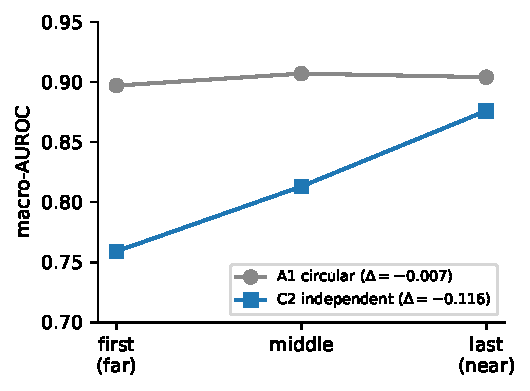
\includegraphics[width=\columnwidth]{distant_window.pdf}
\caption{Distant-window analysis. On the circular target (A1) the gap is $\approx 0$ (leak); on the
independent end-to-end model (C2) AUROC falls as the window moves away from injection,
$\Delta_{\text{far}-\text{near}}=-0.116$ --- genuine temporal precursion.}
\label{fig:distant}
\end{figure}

\subsection{Synthesis and reproducibility caveat}
The encoder's value is \emph{geometric} (it structures the latent space for typing, H1) and
\emph{ontological} (it grounds the OWL artefact), not aggregate-predictive. The honest predictive
contribution is active-scenario typing at $0.920$ with confirmed temporal precursion. A multi-seed
audit (Phase~H/J/K) tempers earlier single-seed optimism: a prior run on seed~42 reported
silhouette $0.84$ and $\Delta=-0.05$, but neither reproduces across ten seeds (silhouette
$0.691\pm0.115$; $\Delta$ leak-confirmed on $9/10$ seeds, seed~42 the lone outlier). The headline
$0.920$ is unaffected because the underlying logistic regression is deterministic; the bootstrap CI
captures its only stochasticity.

\section{Limitations}
\label{sec:limitations}

We documented seventeen limitations (L1--L17); Table~\ref{tab:limitations} lists the structural
ones with their proposed fixes. Four deserve emphasis.

\textbf{Short episodes (L1)} are the dominant data constraint. At $\sim$21 steps, \texttt{ewat\_v3}
leaves too little window for the look-through warm-up, which is the proximate cause of H2a's
failure, H2b's triviality, and the high false-alarm rate at low thresholds. \texttt{ewat\_v4}
(47--51 steps) mitigates but does not eliminate it (H2a still fails).

\textbf{Evaluation circularity (L9)} is the methodological core of this paper. The
$0.987$ precursor AUROC targets EWAT's own labels; we therefore demote it and adopt the independent
Chaos~Mesh target ($0.920$) as the headline, with the stress tests of Section~\ref{sec:validity} as
the evidence.

\textbf{Type-count instability (L10).} The siamese head overfits in $2$--$7$ epochs on
\texttt{ewat\_v4} and $K$ ranges from $9$ to $15$ across seeds; this is structural (small training
set, diverse episode lengths), not a mining bug. We recommend fixing $K$ or moving to density-based
clustering in future iterations.

\textbf{Scope and external validity (L13, L14, L17).} All experiments use one six-service topology
on one cluster. Zero-shot transfer to RCAEval recovers generic anomaly detection (H1 silhouette
$0.684$) but not type discrimination (H3 $\approx 0.5$); the bottleneck is a non-transferable
scaler. The ontology, while HermiT-consistent and literature-anchored, has not been audited by an
operational SRE, and its causal edges are extracted from synthetic cascades.

\begin{table}[t]
\centering
\caption{Structural limitations and proposed fixes.}
\label{tab:limitations}
\small
\begin{tabularx}{\columnwidth}{@{}lXl@{}}
\toprule
\textbf{ID} & \textbf{Limitation} & \textbf{Fix} \\
\midrule
L1  & short episodes ($\sim$21 steps)      & \texttt{v4}/\texttt{v5} long episodes \\
L9  & H3 circularity                        & independent target \\
L10 & siamese overfit / $K$ unstable        & fixed $K$ / HDBSCAN \\
L13 & $N=6$, one topology                   & Train~Ticket (\texttt{v5}) \\
L14 & no cross-cluster validation           & few-shot domain adapt. \\
L17 & ontology not SRE-audited              & expert review \\
\bottomrule
\end{tabularx}
\end{table}

We also note minor caveats for transparency: a single train/val/test split (no $k$-fold), no a
priori power analysis (post-hoc: $5/10$ clusters are statistically reportable at $n_{\text{pos}}\geq
5$), and stress tests A1--A5 designed \emph{post hoc} rather than pre-registered.

\section{Discussion and Future Work}
\label{sec:discussion}

\paragraph{What EWAT is, and is not.}
EWAT is a working early-warning pipeline whose honest, independently-validated contribution is
active-scenario typing at $0.920$ macro-AUROC with confirmed temporal precursion
($\Delta=-0.116$). It is not a generic event predictor: the learned encoder adds geometric and
ontological value, not aggregate predictive power, and open-set generalisation to unseen fault
types remains only partially solved. We consider the negative and nuanced results --- a robustly
falsified look-through, a circular metric demoted in favour of an independent one, an unstable type
count --- to be as much a contribution as the positive headline, because they delimit precisely
where the approach is and is not trustworthy.

\paragraph{Roadmap.}
Four research axes follow directly from the limitations.
\emph{Axis~A (ontology$\,\leftrightarrow\,$prediction coupling)} would feed the causal graph back
into the precursor as upstream features or a post-hoc re-ranker, testing whether the ontology adds
predictive value rather than only descriptive value.
\emph{Axis~B (robust temporal precursion)} would replace the STGCN with a temporal transformer,
multi-seed the C2 distant-window result, and validate lead time cross-dataset on RCAEval.
\emph{Axis~C (open-set)} would extend the partial OpenMax result with Mahalanobis-based and
energy-based detectors and few-shot meta-learning.
\emph{Axis~D (deployment)} would specify the streaming pipeline, the retraining trigger, and a
formal alert contract.

\paragraph{Towards \texttt{ewat\_v5}.}
The most consequential next step is data. \texttt{ewat\_v5} abandons the six-service Online Boutique
for \emph{Train~Ticket} (41 Spring~Cloud services), with a much larger episode budget and, crucially,
a held-out set drawn from the project's documented \emph{real} bugs (the F1--F12 catalogue) ---
a literature gold standard for RCA-style evaluation. This directly attacks L1 (episode length),
L13 (topology scale), L14 (cross-system validity), and L17 (real rather than synthetic faults),
and would let us re-test every hypothesis on a substantially harder and more realistic system.

\section{Conclusion}
\label{sec:conclusion}

EWAT shows that benign drift and genuine anomalies can be separated and that developing faults can
be typed ahead of time in a real Kubernetes microservice environment, provided the four operational
regimes --- including the combined $\thetadn$ --- are modelled explicitly. Our two robust positive
results are geometric structurability (H1, silhouette $0.782\pm0.065$ over ten seeds) and, against
an \emph{independent} ground truth, active-scenario typing at macro-AUROC $0.920$ $[0.878,0.956]$
with confirmed temporal precursion ($\Delta_{\text{far}-\text{near}}=-0.116$) and a $13$~ms p95
latency. We deliberately refuse the inflated self-referential number ($0.987$) and the
single-seed optimism it came with, and we report the look-through falsification and the partial
open-set result as honest negatives that constrain future work rather than embarrassments to be
hidden. The path forward is more and harder data: \texttt{ewat\_v5} on Train~Ticket with real,
documented faults will let us re-test every hypothesis at production scale.


\printbibliography[heading=bibintoc, title={References}]

\appendix
\section{Per-cluster precursor results}
\label{app:precursor}

Table~\ref{tab:percluster} gives the per-type precursor results on \texttt{ewat\_v3} (seed 42,
$k^*$ selected on validation, AUROC on test with $95\%$ bootstrap CI). These are
\emph{circular}-target numbers (Section~\ref{sec:results}) and should be read alongside the
stress-test caveats of Section~\ref{sec:validity}. Clusters with fewer than two positive test
episodes (C6, C9) yield undefined AUROC and are marked n/a.

\begin{table}[h]
\centering
\caption{Per-cluster precursors (\texttt{ewat\_v3}, circular target). $k^*$ in 30~s steps.}
\label{tab:percluster}
\small
\begin{tabularx}{\columnwidth}{@{}lrrrX@{}}
\toprule
\textbf{Type} & $n_{\text{pos}}$ & $k^*$ & \textbf{AUROC} & \textbf{95\% CI} \\
\midrule
C0 & 8 & 6  & 0.973 & [0.906, 1.000] \\
C1 & 3 & 6  & 0.992 & [0.953, 1.000] \\
C2 & 5 & 6  & 0.945 & [0.865, 1.000] \\
C3 & 3 & 2  & 0.794 & [0.636, 0.930] \\
C4 & 8 & 2  & 1.000 & [1.000, 1.000] \\
C5 & 2 & 6  & 0.977 & [0.909, 1.000] \\
C6 & 1 & 2  & n/a   & --- \\
C7 & 7 & 6  & 0.992 & [0.966, 1.000] \\
C8 & 7 & 10 & 0.962 & [0.895, 1.000] \\
C9 & 1 & 2  & n/a   & --- \\
\bottomrule
\end{tabularx}
\end{table}

The dominant optimal horizon is $k^*=6$ steps ($3$~min), the practical zone of predictability for
most fault types in this dataset; \texttt{C3} has an immediate signature ($k^*=2$) and \texttt{C8}
(the combined-regime overlap) a slow one ($k^*=10$).

\section{Cluster--scenario alignment}
\label{app:nmi}

Normalised mutual information between clusters and Chaos~Mesh scenarios is $0.518$ and mean purity
$0.503$ --- the moderate alignment expected of unsupervised clustering that compresses 15 scenarios
into $\approx 10$ empirical types. Two scenarios sharing a latent fault signature (e.g.\ crash and
OOM near the injection point) are a finding, not an error. Figure~\ref{fig:heatmap} shows the
full alignment. Gradient$\times$input saliency was found unreliable ($\rho=-0.34$ versus
permutation importance) and is not used; permutation importance is cross-validated by KernelSHAP
($\rho>0$ on $9/10$ clusters).

\begin{figure}[h]
\centering
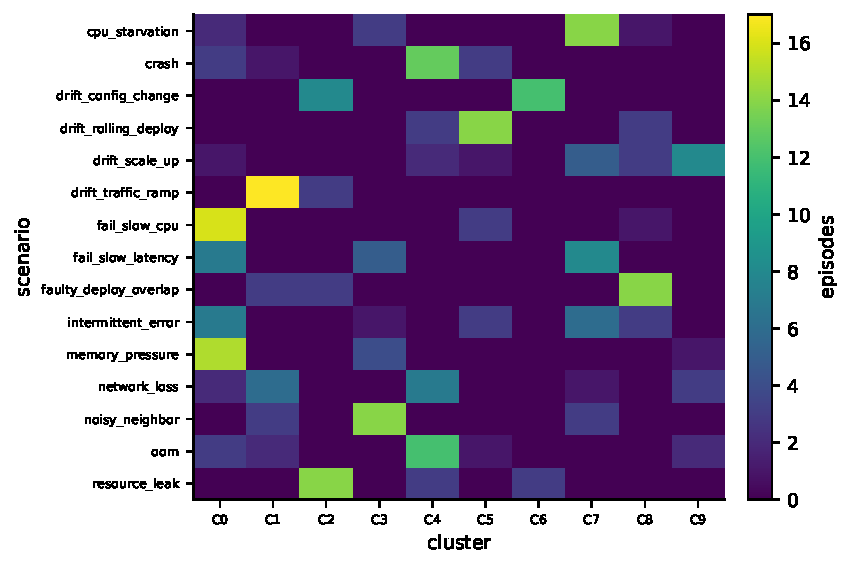
\includegraphics[width=\columnwidth]{scenario_cluster_heatmap.pdf}
\caption{Scenario$\times$cluster alignment heatmap (\texttt{ewat\_v3}).}
\label{fig:heatmap}
\end{figure}


\end{document}
